\documentclass[a4paper,11pt]{article}
\input{/home/tof/Documents/Cozy/latex-include/preambule_doc.tex}
\input{/home/tof/Documents/Cozy/latex-include/preambule_commun.tex}
\newcommand{\showprof}{show them}  % comment this line if you don't want to see todo environment
\setlength{\fboxrule}{0.8pt}
\fancyhead[L]{\fbox{\Large{\textbf{Loc 02}}}}
\fancyhead[C]{\textbf{Géoportail}}
\newdate{madate}{10}{09}{2020}
%\fancyhead[R]{\displaydate{madate}} %\today
\fancyhead[R]{Seconde - SNT}
\fancyfoot[L]{\vspace{1mm}Christophe Viroulaud}
\AtEndDocument{\label{lastpage}}
\fancyfoot[C]{\textbf{Page \thepage/\pageref{lastpage}}}
\fancyfoot[R]{\includegraphics[width=2cm,align=t]{/home/tof/Documents/Cozy/latex-include/cc.png}}

\begin{document}
\begin{center}
    \framebox{Quelles sont les fonctionnalités du Géoportail?}
\end{center}
\section{L'IGN}
\subsection{Mission}
\begin{center}
    {\Large Observer - Mesurer - Décrire le territoire}
\end{center}
Le rôle de l'IGN est de fournir des données géolocalisées fiables et de favoriser leur utilisation.
\subsection{Moyens technologiques}
L'IGN utilise de nombreux moyens pour récolter l
les données:
\begin{itemize}
    \item \textbf{Géoplateforme}: mutualisation des données entre l'IGN et ses partenaires,
    \item \textbf{Lidar HD}: relevé laser de grande précision
    \item \dots
\end{itemize}
\section{Géoportail}
Le Géoportail est un site web qui permet d'accéder aux données fournies par l'IGN.
\begin{center}
\centering
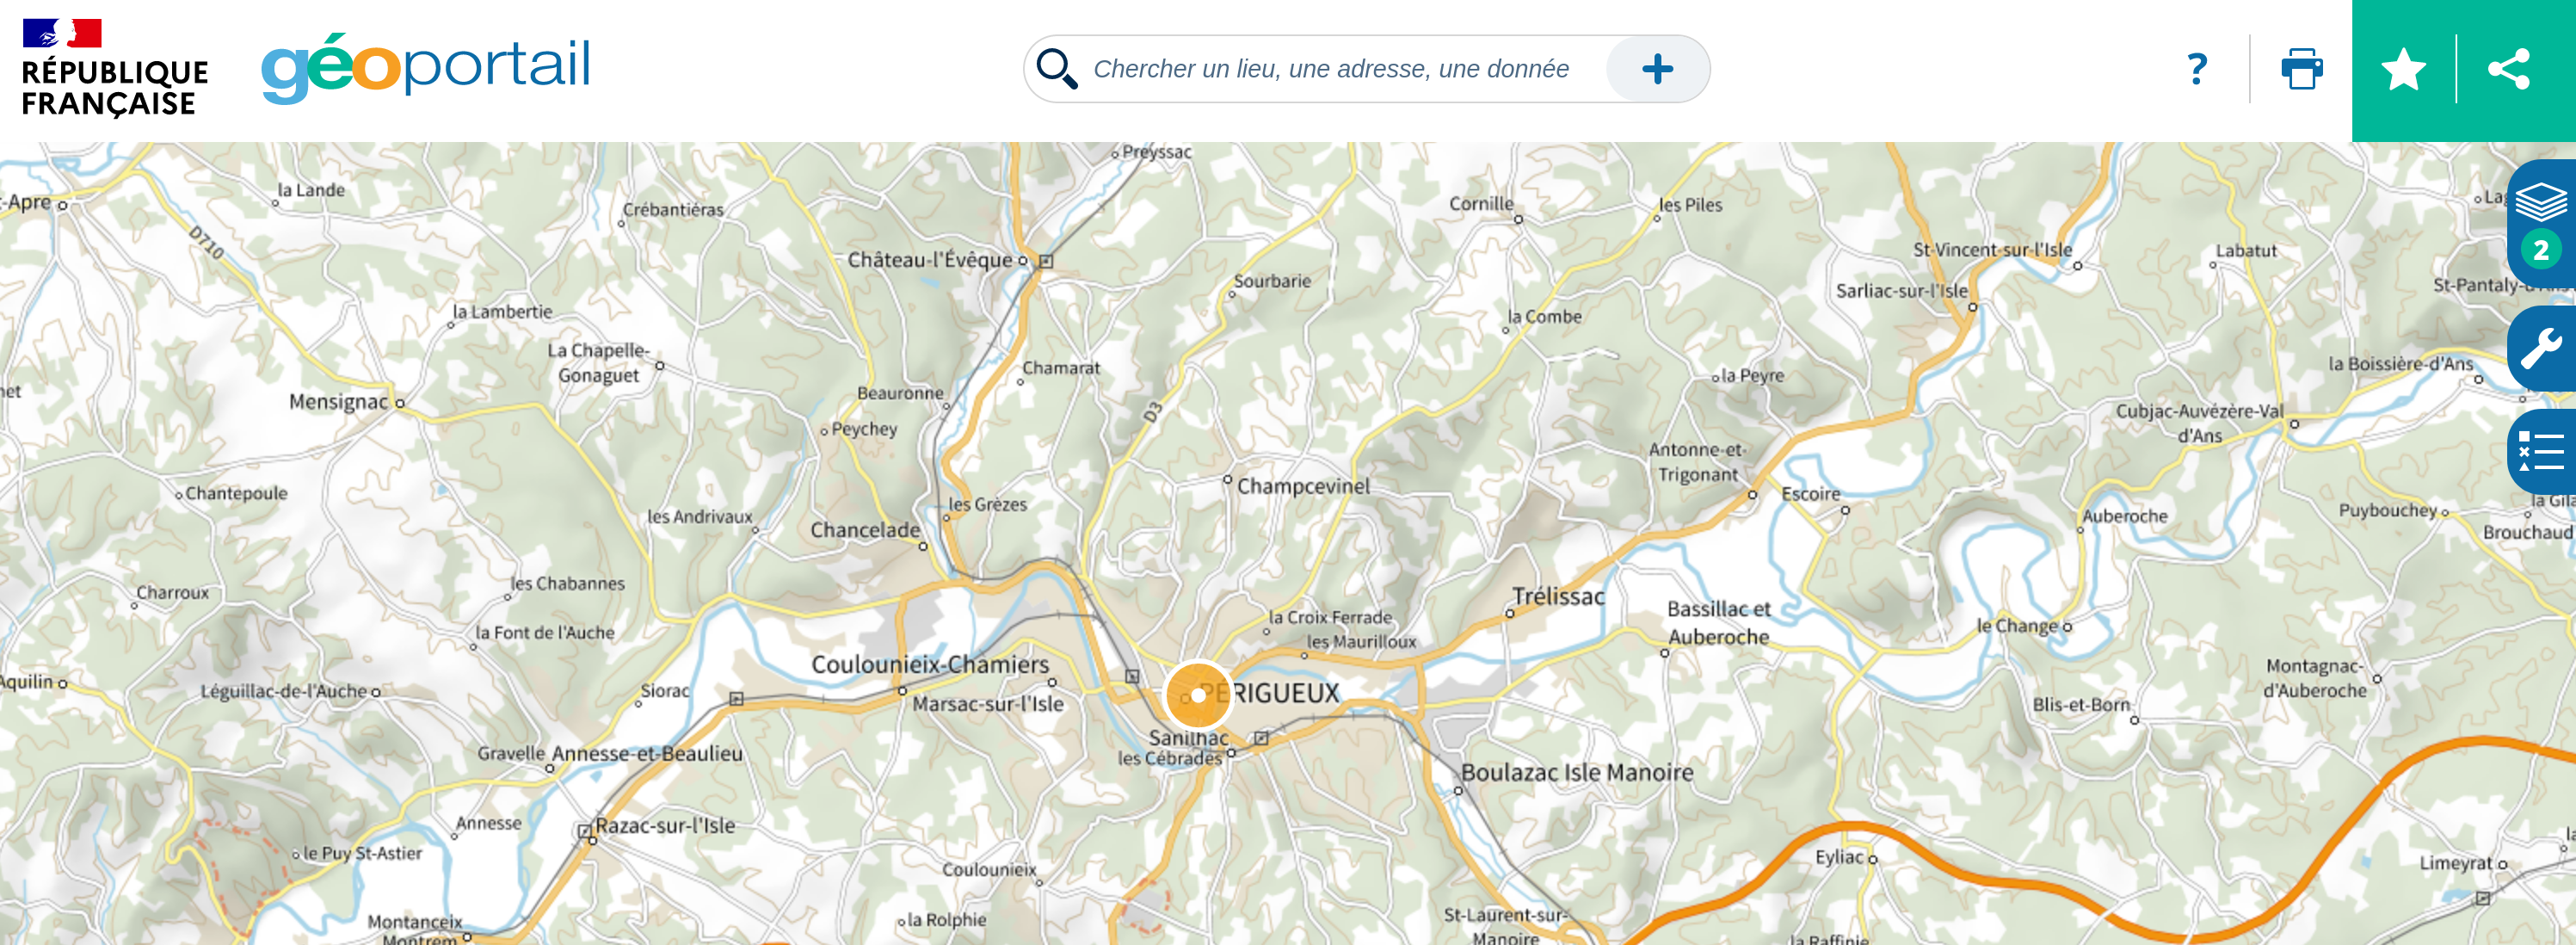
\includegraphics[width=10cm]{ressources/geoportail.png}
\end{center}
Il existe de nombreux fonds de cartes qui fournissent des informations différentes (lignes de niveau, cadastre\dots)
\begin{center}
\centering
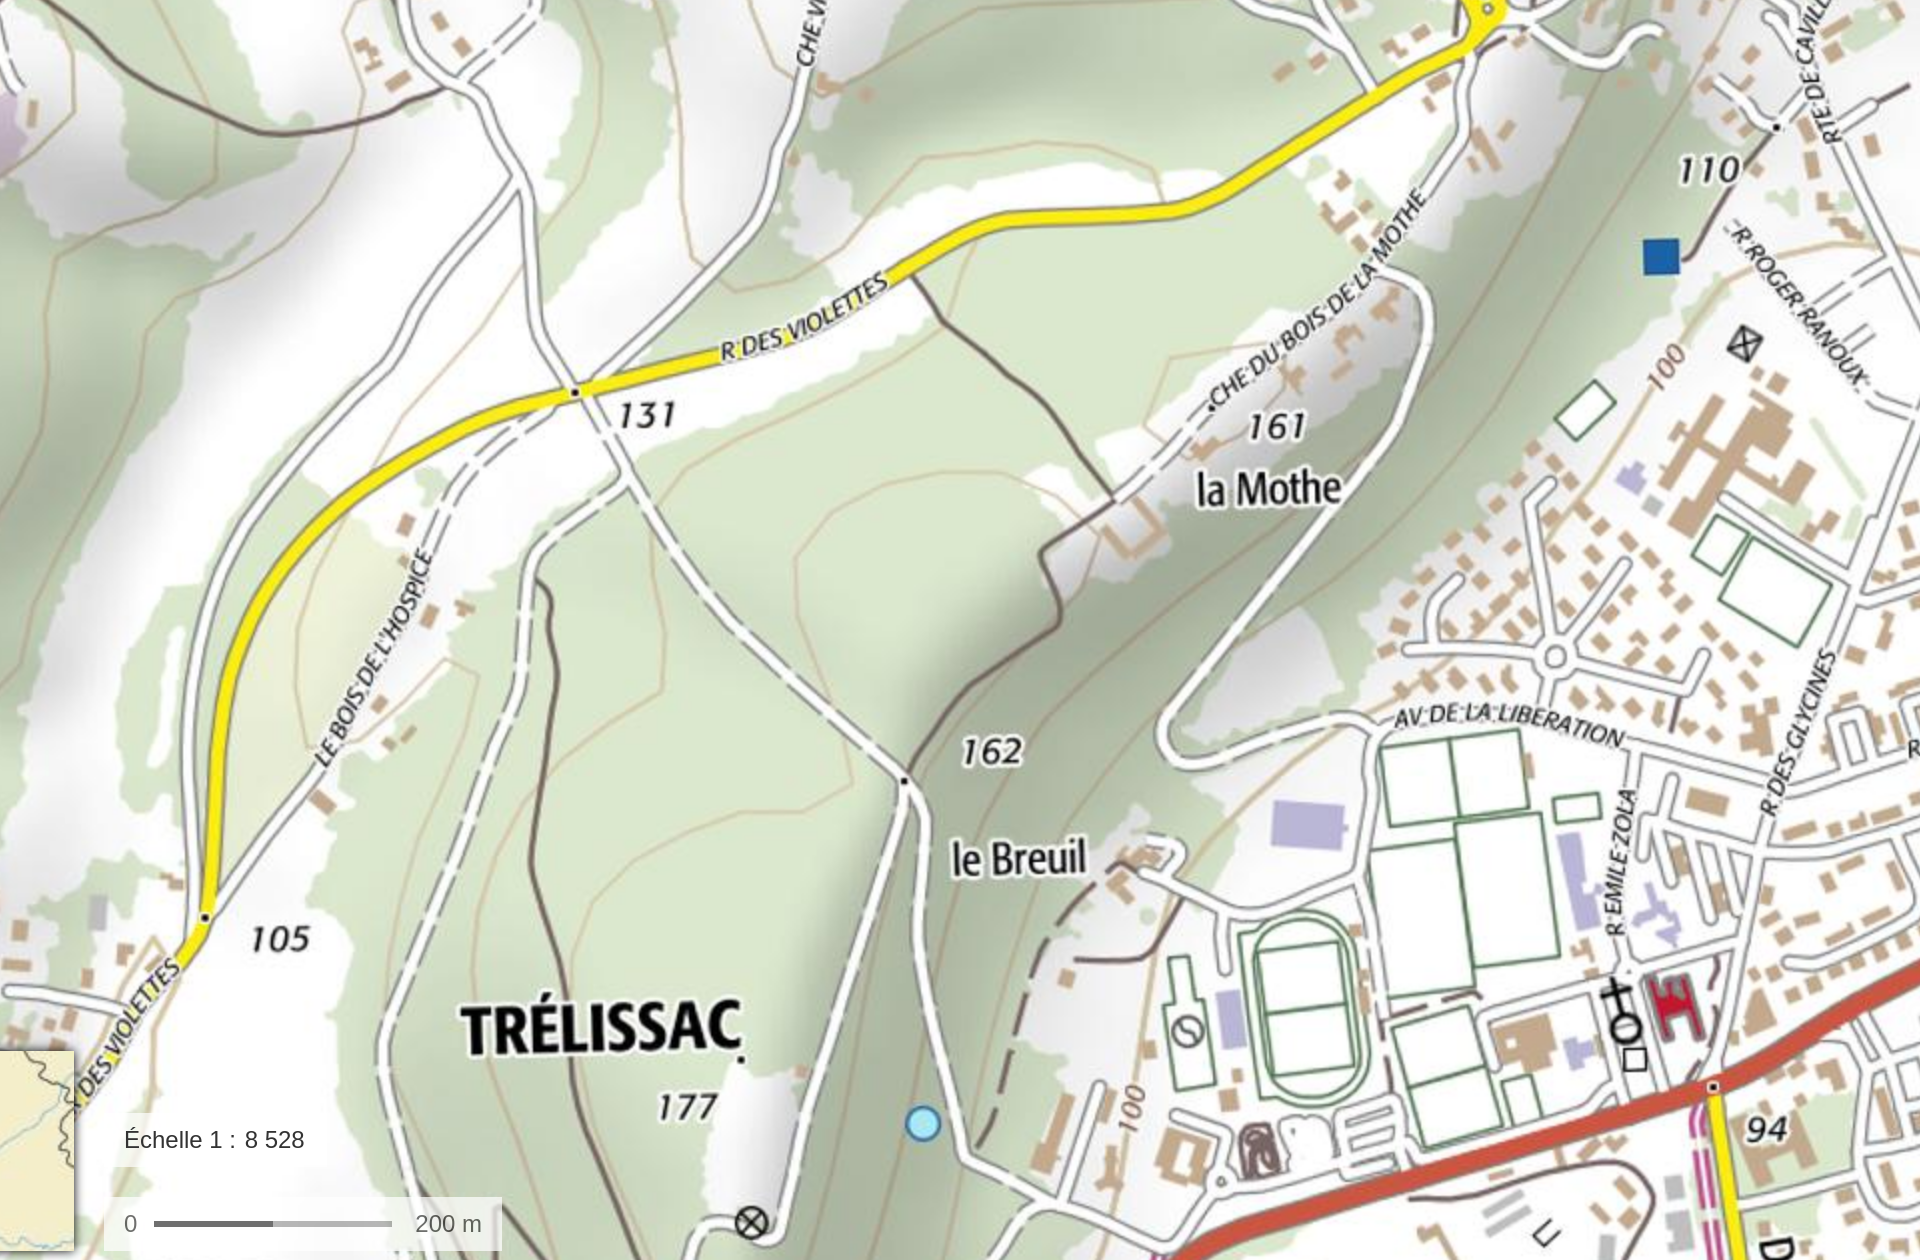
\includegraphics[width=8cm]{ressources/mission-ign.png}
\end{center}
\end{document}